\documentclass[aspectratio=169]{beamer}
\usetheme{Madrid}
\usecolortheme{beaver}
\usepackage[utf8]{inputenc}
\usepackage[T1]{fontenc}
\usepackage{tikz}
\usepackage{amssymb}
\usepackage{graphicx}
\setbeamertemplate{navigation symbols}{}
\setbeamercolor{title}{fg=white,bg=cyan!60!black}
\setbeamercolor{frametitle}{fg=white,bg=cyan!50!black}
\setbeamercolor{block title}{bg=cyan!15,fg=black}
\setbeamercolor{block body}{bg=cyan!5,fg=black}

\title{G5 — Player Control}
\subtitle{Lesson 2: Aim with the Mouse}
\author{ByteForge --- Grade 7 --- Game Maker}
\date{}

\begin{document}

\begin{frame}
    \titlepage
\end{frame}

\begin{frame}{Mouse position — always available, live}
    \Large
    mouseX()/mouseY() always report the CURRENT position, live — nothing to set or update, the engine tracks it automatically.

    \begin{center}
    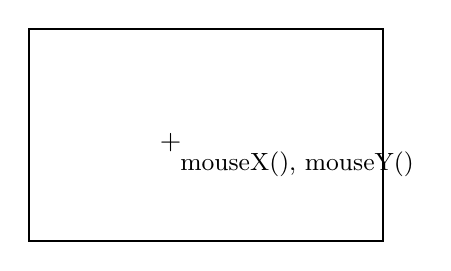
\begin{tikzpicture}[scale=0.9]

        \draw[thick] (0,0) rectangle (5,-3);
        \node at (2,-1.6) {$+$};
        \node[below right] at (2,-1.6) {\small mouseX(), mouseY()};
    \end{tikzpicture}
    \end{center}
\end{frame}

\begin{frame}{Your Turn}
    \Large
    Open the student map, find \textbf{G5 — Player Control}, and complete
    the \textbf{Aim with the Mouse} challenge --- everything you just saw, they now do themselves.
\end{frame}

\end{document}
